\section{Core-Modul}
\label{sec:coremodul}

\fig{core-modul}{Core-Modul}{\gls{Core-Modul}}{\textwidth}{Schuh/Pictures/coremodul}

\subsection{Allgemeines}
\label{sec:coremodul-allgemeines}

Das \gls{Core-Modul} ist das Herzstück des gesamten \gls{ARM}-\gls{Minimalsystem}s, denn auf diesem befindet sich der Prozessor und alle Komponenten welche für den ordnungsmäßigen Betrieb erforderlich sind. Die einzelnen Port-Pins des Prozessors sind entweder direkt auf dem \gls{Core-Modul} verwendet oder über externe Anschlüsse nach außen geführt. Weiters verfügt das \gls{Core-Modul} über alle nötigen Programmierschnittstellen um unabhängig von der \gls{Basisplatine} oder anderen Programmierplatinen programmiert und verwendet werden zu können. Darüber hinaus kann mit der auf dem \gls{Core-Modul} befindlichen UART-Schnittstelle eine direkte Kommunikation mit anderen Modulen oder einem Terminal aufgebaut werden.

\subsection{Schnittstellen}
\label{sec:coremodul-schnittstellen}

In \fref{tab:coremodul-schnittstellen} sind die verfügbaren Schnittstellen des \gls{Core-Modul}s aufgelistet. In \fref{fig:coremodul-plan} ist dargestellt, wo auf der Platine die einzelnen Schnittstellen platziert sind.

\tab{coremodul-schnittstellen}{Schnittstellen des Core-Moduls}{Schnittstellen des \gls{Core-Modul}s}{|c|p{10cm}|}{
    \hline
    \textbf{Schnittstelle} & \textbf{Funktion}\\
    \hline
    USART 1 & Universal Synchronous/Asynchronous Receiver/Transmitter, Datenübertragung\\
    \hline
    SWD & \gls{SWD}, Programmierung\\
    \hline
    ST-Link V2 & Programmierung auf Basis von \gls{SWD}\\
    \hline
    50 poliger Header & Ausführung der Port-Pins auf die \gls{Basisplatine}\\
    \hline
}

\fig{coremodul-plan}{Übersichtsplan des Core-Moduls}{Übersichtsplan des \gls{Core-Modul}s}{0.75\textwidth}{Schuh/Pictures/Core}

\subsection{Prozessor}
\label{sec:coremodul-prozessor}

Als Prozessor für das \gls{Core-Modul} wurde der \gls{cpu} von der Firma \gls{STM} verwendet. Die Key-Features sind in \fref{fig:coremodul-features} zusammengefasst.

\fig{coremodul-features}{Features des Prozessors}{Features des Prozessors \cite{stm:stm32f107rc-web}}{\textwidth}{Schuh/Pictures/Features}

\subsubsection{Blockschaltbild}
Im Gegensatz zum bisher verwendeten STM32F103RB verfügt der \gls{cpu} über zwei \IIS{}-Schnittstellen, welche für den Audioadapter (\fref{sec:audioadapter}) verwendet werden. Des weiteren verfügt der neue Microcontroller einen \gls{DAC}, einen Ethernet-Controller (MAC) und ist USB OTG-fähig.
\fig{coremodul-cpubsb}{Blockschaltbild des Prozessors}{Blockschaltbild des Prozessors \cite{stm:stm32f107rc}}{\textwidth}{Schuh/Pictures/BSB}

\subsubsection{Pinning}
\fig{coremodul-cpupinning}{Pinning des Prozessors}{Pinning des Prozessors \cite{stm:stm32f107rc}}{\textwidth}{Schuh/Pictures/Pinning}

\subsubsection{Abmessungen}
\fig{coremodul-cpumeasure}{Abmessungen des Prozessors}{Abmessungen des Prozessors \cite{stm:stm32f107rc}}{0.8\textwidth}{Schuh/Pictures/MeasureGraphic}
\tabpdf{coremodul-cpumeasure}{Abmessungen des Prozessors}{Abmessungen des Prozessors \cite{stm:stm32f107rc}}{0.8\textwidth}{Schuh/Pictures/MeasureTable}

\subsubsection{Pinbelegung}
\begin{table}[H]
    \centering
    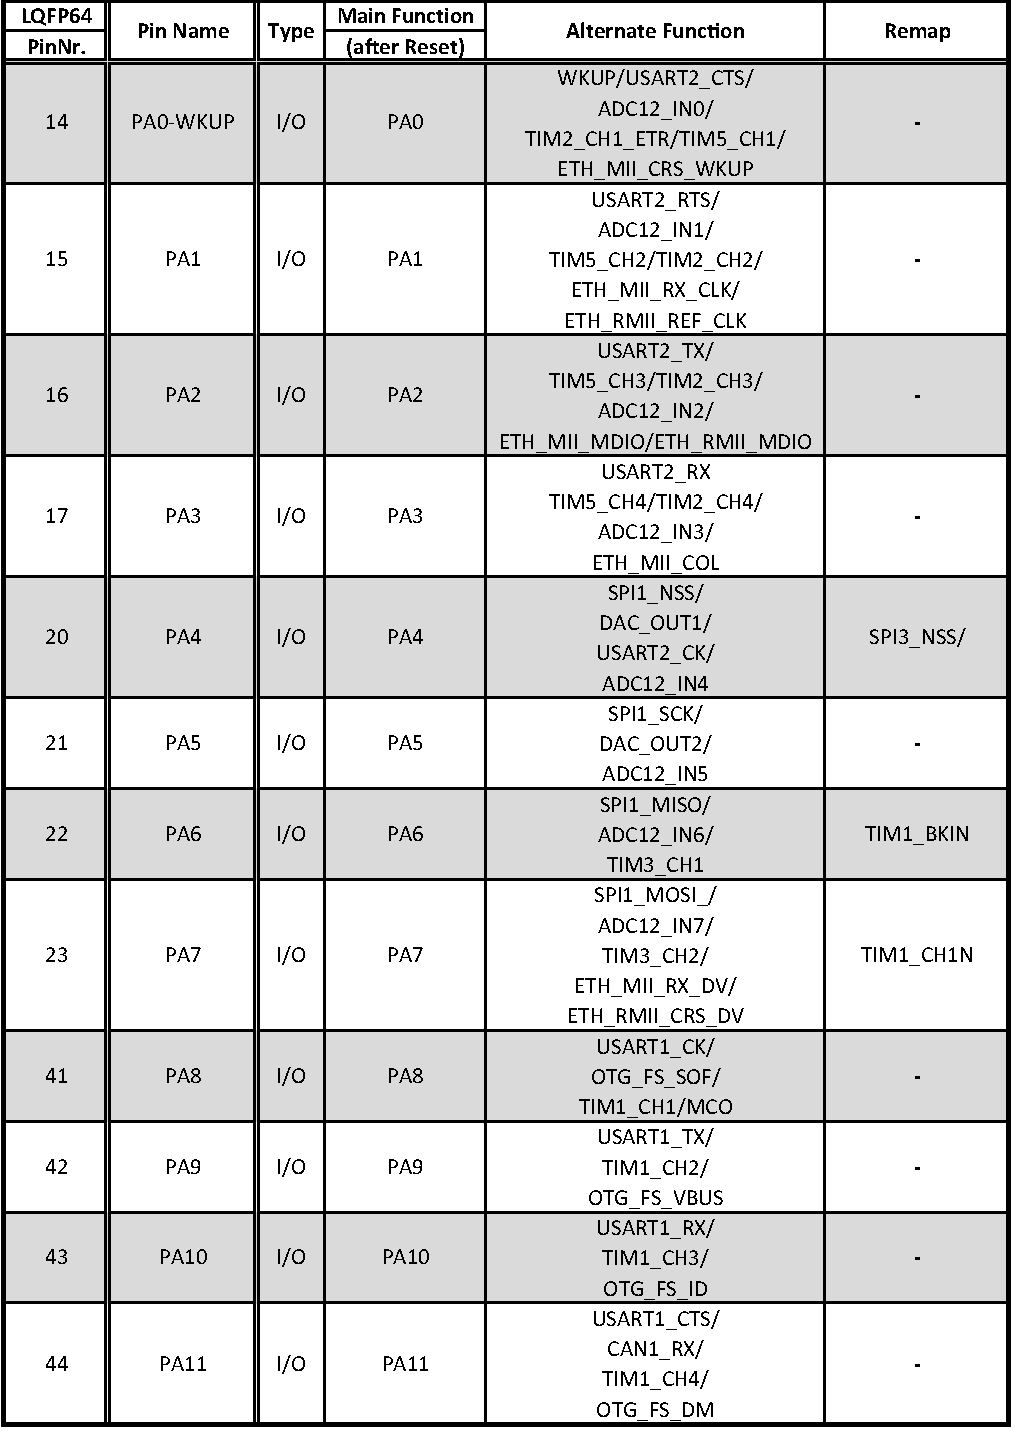
\includegraphics[width=0.9\textwidth]{Schuh/Pictures/Pinbelegung1}
    \caption[Pinbelegung des Prozessors]{Pinbelegung des Prozessors \cite{stm:stm32f107rc}}
    \label{tab:coremodul-cpupins}
\end{table}
\begin{table}[H]\ContinuedFloat
    \centering
    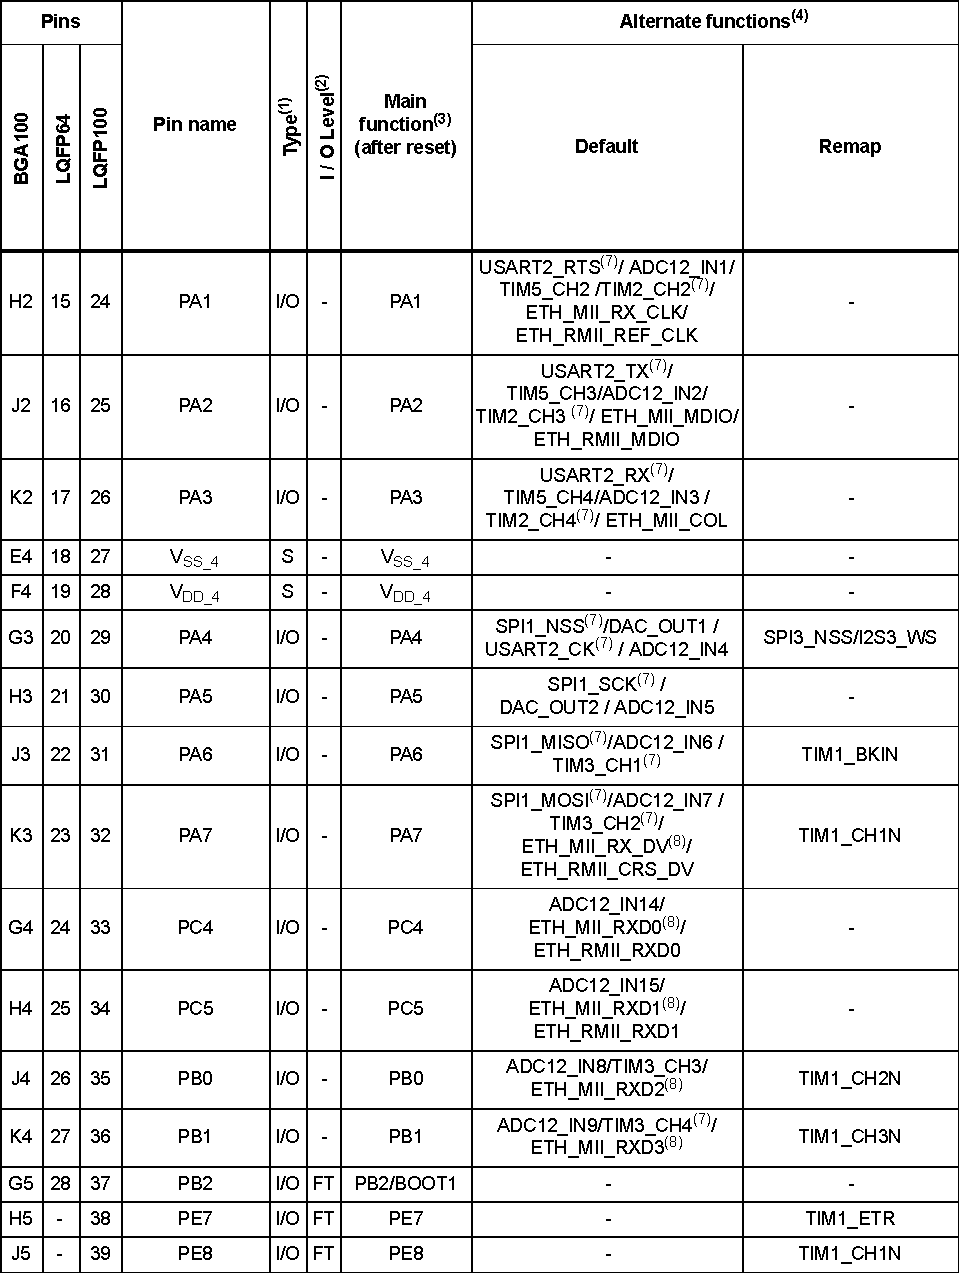
\includegraphics[width=0.9\textwidth]{Schuh/Pictures/Pinbelegung2}
    \caption[Pinbelegung des Prozessors]{Pinbelegung des Prozessors \cite{stm:stm32f107rc}}
\end{table}
\begin{table}[H]\ContinuedFloat
    \centering
    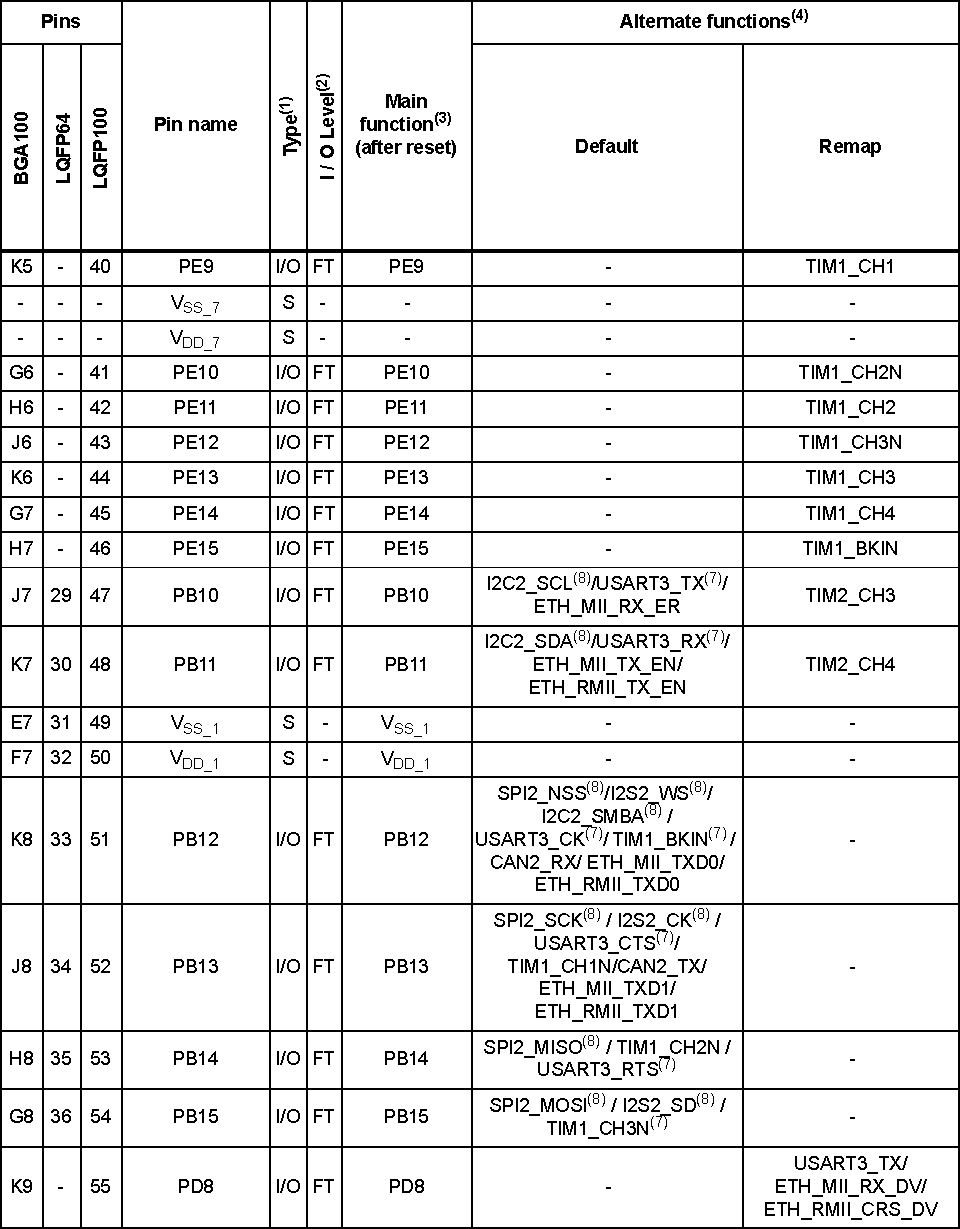
\includegraphics[width=0.9\textwidth]{Schuh/Pictures/Pinbelegung3}
    \caption[Pinbelegung des Prozessors]{Pinbelegung des Prozessors \cite{stm:stm32f107rc}}
\end{table}
\begin{table}[H]\ContinuedFloat
    \centering
    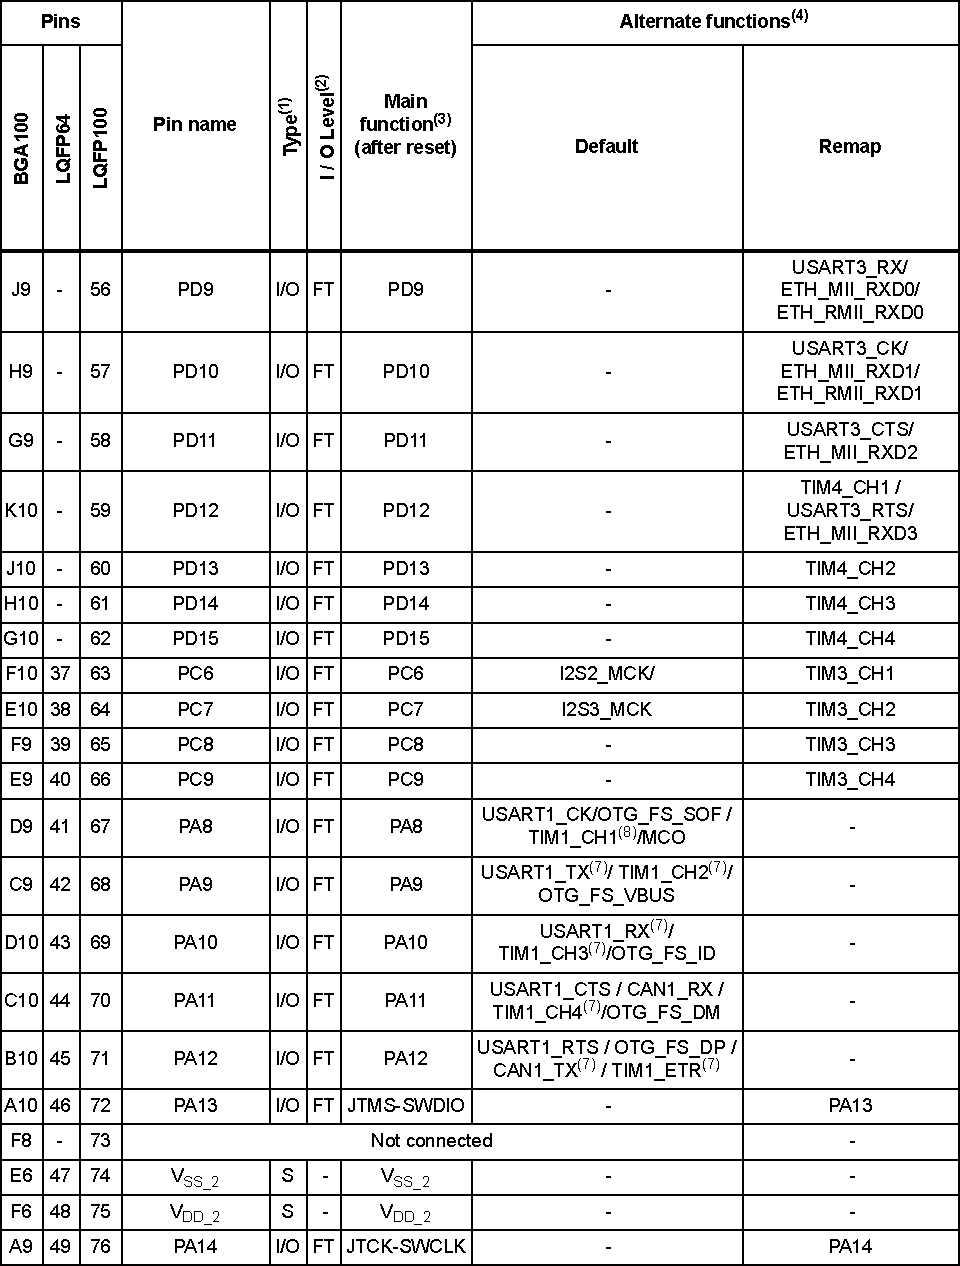
\includegraphics[width=0.9\textwidth]{Schuh/Pictures/Pinbelegung4}
    \caption[Pinbelegung des Prozessors]{Pinbelegung des Prozessors \cite{stm:stm32f107rc}}
\end{table}
\begin{table}[H]\ContinuedFloat
    \centering
    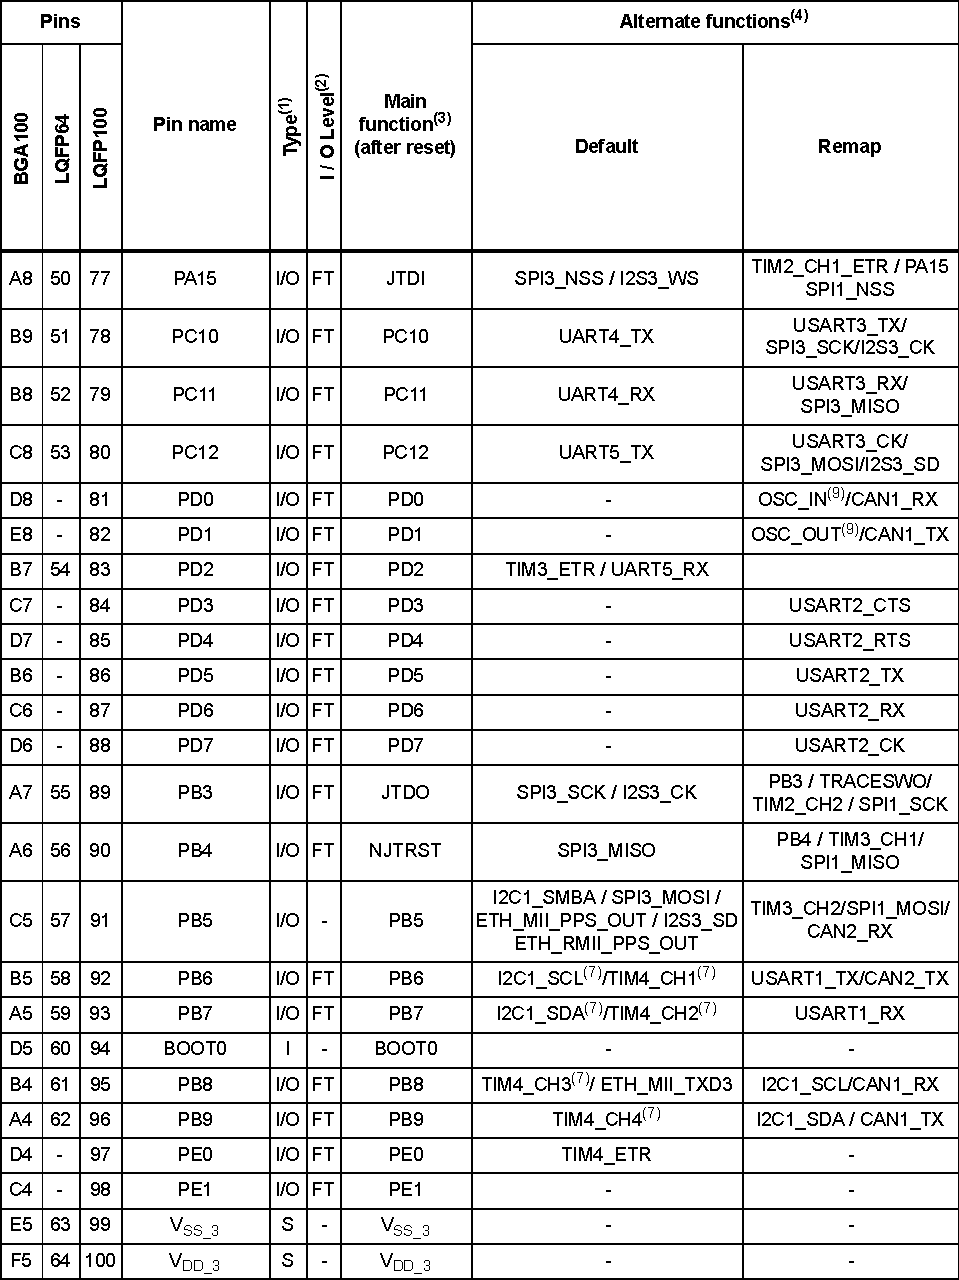
\includegraphics[width=0.9\textwidth]{Schuh/Pictures/Pinbelegung5}
    \caption[Pinbelegung des Prozessors]{Pinbelegung des Prozessors \cite{stm:stm32f107rc}}
\end{table}

\subsection{Portbelegungsplan}
\label{sec:coremodul-portbelegung}
\tabpdf{coremodul-portbelegung}{Portbelegungsplan des Core-Moduls}{Portbelegungsplan des \gls{Core-Modul}s}{0.55\textwidth}{Schuh/Pictures/Portbelegung}

\subsubsection{Programmierung mit ST-Link V2}
\label{sec:coremodul-stlink}
Zur Programmierung und zum \gls{Debugging} des neuen \gls{ARM}-\gls{Minimalsystem}s sollte ein \textbf{ST-Link V2 Mini} (\fref{fig:coremodul-stlink}) verwendet werden. Dieser Programmer besitzt eine verpolungssichere zweireihige Stiftreihe, welche es ermöglicht Programme mit Hilfe von \gls{SWD} auf den Microcontroller zu übertragen oder diese zu debuggen. Darüber hinaus ist der ST-Link V2 Mini der Lieferant der Hauptversorgungsspannung von \unit{+5}{\volt}.

Um den ST-Link V2 Mini und den Microcontroller im Falle eines Kurzschlusses zwischen der Versorgungsspannung und Masse zu schützen wurde eine Schottky-Diode V1 (\fref{fig:coremodul-swd}), mit einem maximalen Durchflussstrom von \unit{1}{\ampere}, vorgesehen. Um die Verpolungssicherheit des ST-Link V2 Mini zu gewährleisten, wurde eine zweireihige Buchsenleiste mit Nase X1 (\fref{fig:coremodul-swd}; \fref{fig:coremodul-stlinkbuchse}) verbaut, welche eine Verpolung des ST-Links unmöglich macht.

\fig{coremodul-stlink}{ST-Link V2 Mini}{ST-Link V2 Mini}{0.5\textwidth}{Schuh/Pictures/STLink}

\begin{figure}[H]
    \centering
    \subfloat[Schematic\label{fig:coremodul-swd-schem}]{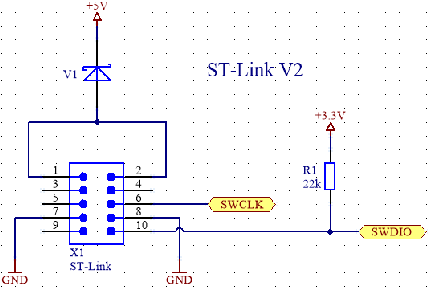
\includegraphics[width=.4\linewidth]{Schuh/Pictures/SchaltungSWD}}\qquad
\subfloat[Hardware\label{fig:coremodul-swd-hard}]{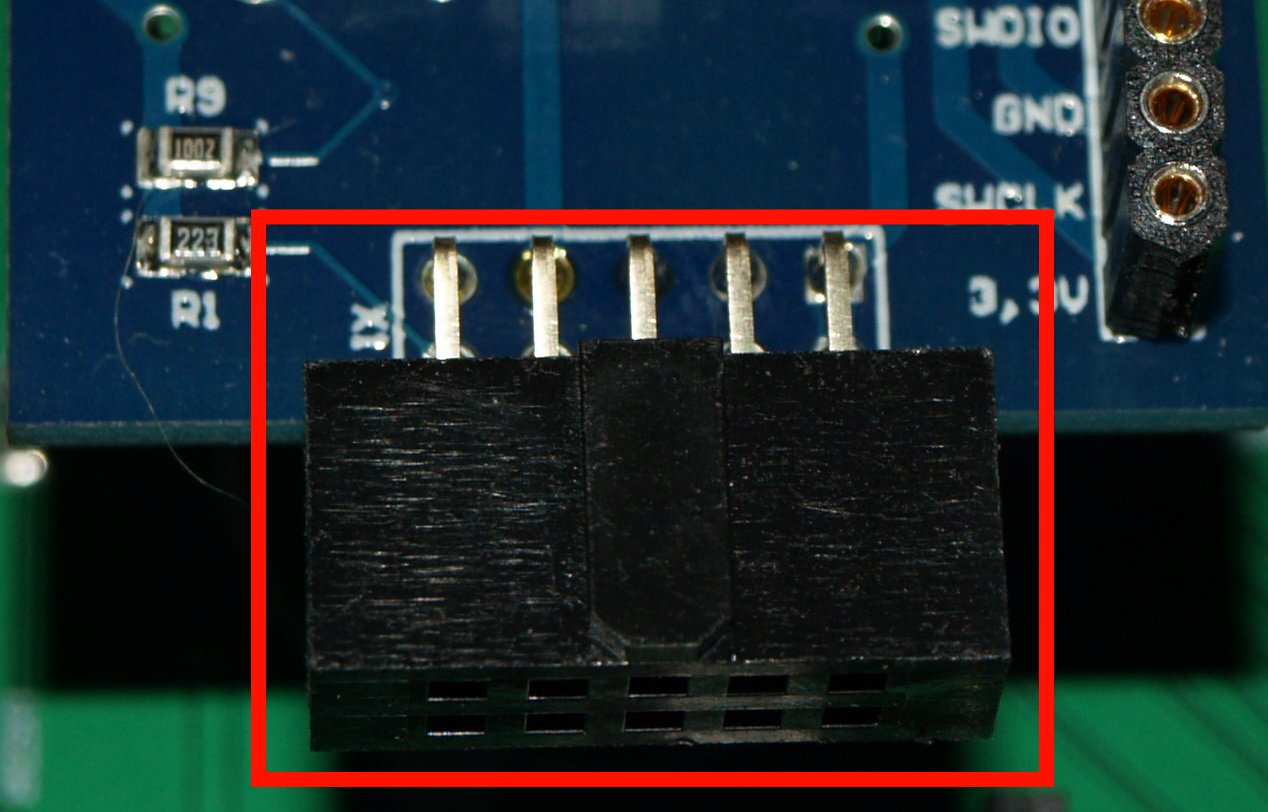
\includegraphics[width=.4\linewidth,angle=270]{Schuh/Pictures/core-stlink}}\qquad
    \caption[ST-Link Schaltung des Core-Moduls]{ST-Link Schaltung des \gls{Core-Modul}s}
    \label{fig:coremodul-swd}
\end{figure}

\fig{coremodul-stlinkbuchse}{Buchse mit Nase}{Buchse mit Nase}{0.5\textwidth}{Schuh/Pictures/STLinkBuchse}

\subsubsection{Single Wire Debug (SWD) Adapter}
Der als Buchsenleiste ausgeführte SWD-Adapter X4 (\fref{fig:coremodul-swd2}), erfüllt vom Prinzip her die gleiche Funktion wie der bereits in \fref{sec:coremodul-stlink} beschriebene Stecker für den ST-Link V2 Mini. Dieser ermöglicht lediglich Kompatibilität zu anderen SWD-Programmern und Debuggern, welche diesen Stecker nicht besitzen.

\begin{figure}[H]
    \centering
    \subfloat[Schematic\label{fig:coremodul-swd2-schem}]{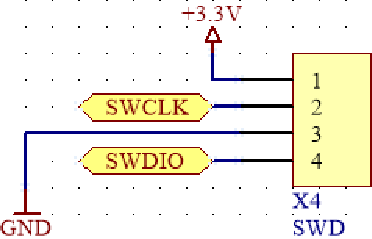
\includegraphics[width=.4\linewidth]{Schuh/Pictures/SchaltungSWD2}}\qquad
    \subfloat[Hardware\label{fig:coremodul-swd2-hard}]{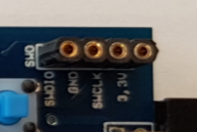
\includegraphics[width=.4\linewidth]{Schuh/Pictures/core-swd}}\qquad
    \caption[SWD-Schaltung des Core-Moduls]{SWD-Schaltung des \gls{Core-Modul}s}
    \label{fig:coremodul-swd2}
\end{figure}

\subsubsection{Serielle Schnittstelle (USART1)}
Die Buchsenleiste X3 (\fref{fig:coremodul-uart}) dient hauptsächlich zur seriellen Kommunikation. Die Pinanordnung wurde so gewählt, dass die Kommunikation entweder kabelgebunden, über den \gls{USB-to-UART} Adapter, oder alternativ über ein HC-06 Bluetooth Modul erfolgen kann.

\begin{figure}[H]
    \centering
    \subfloat[Schematic\label{fig:coremodul-uart-schem}]{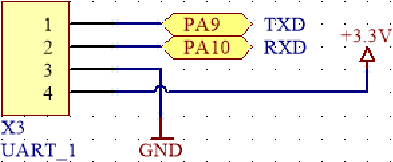
\includegraphics[width=.4\linewidth]{Schuh/Pictures/SchaltungUART}}\qquad
    \subfloat[Hardware\label{fig:coremodul-uart-hard}]{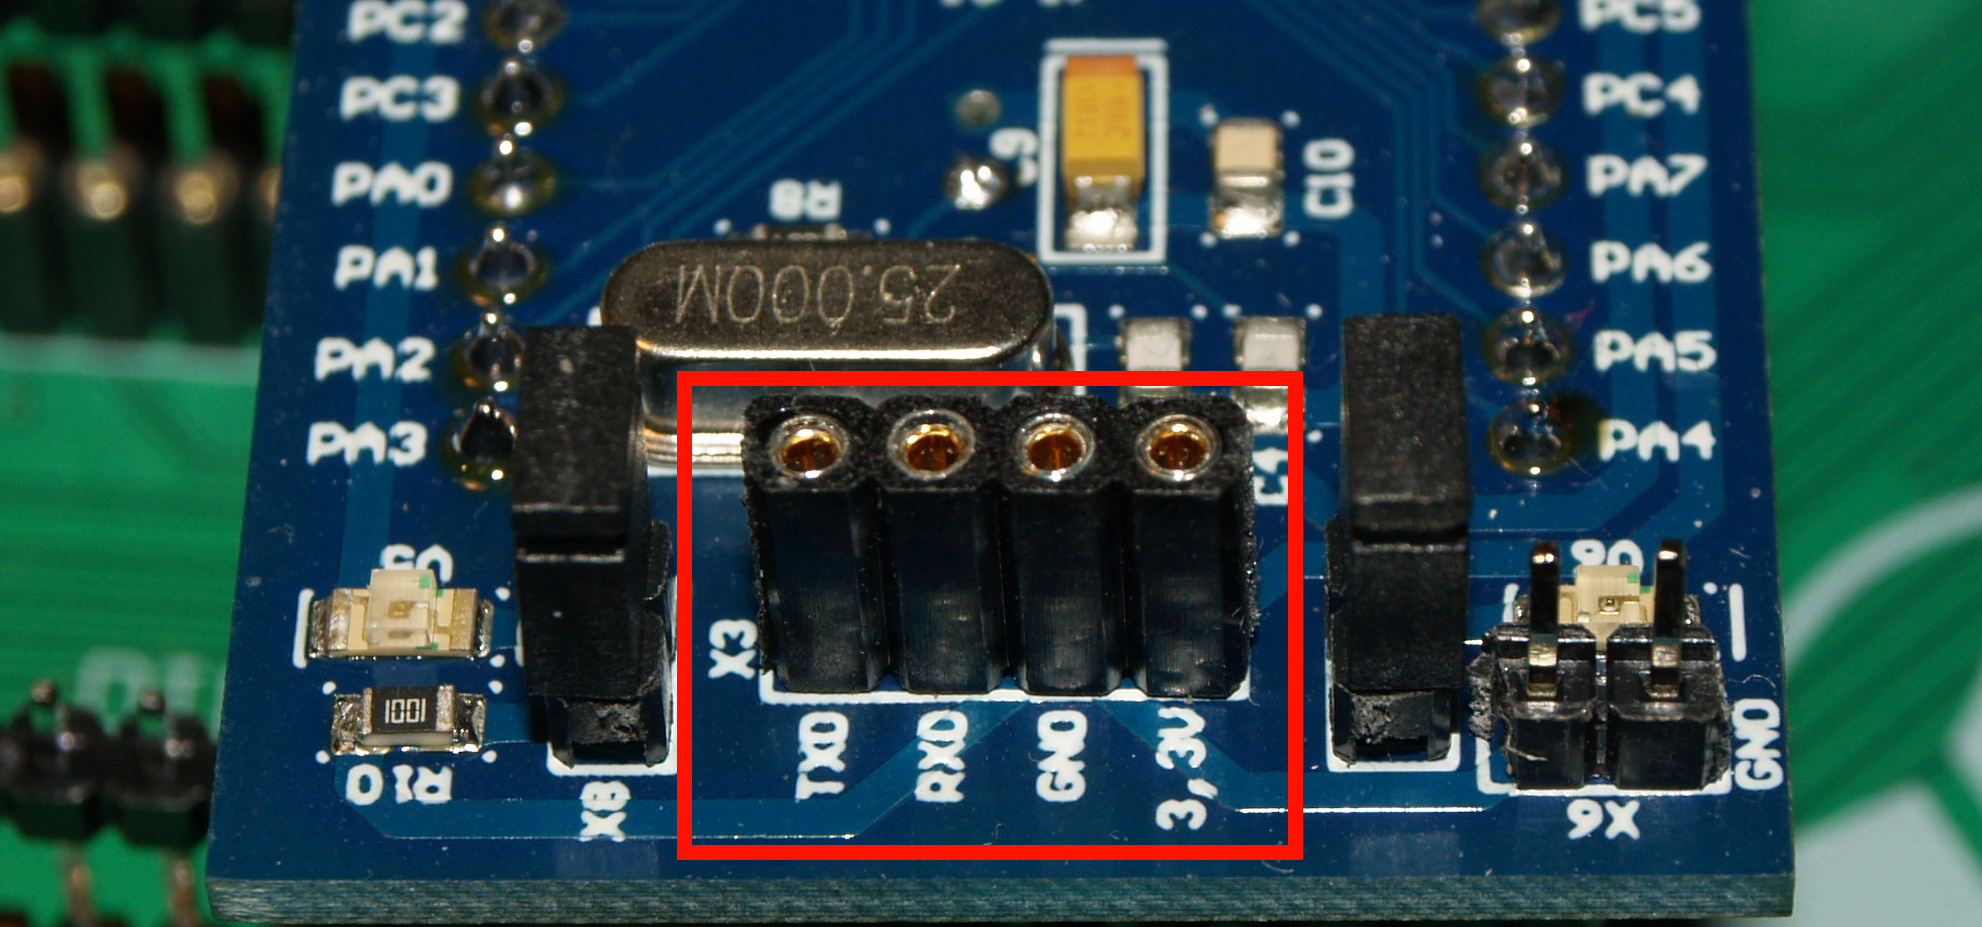
\includegraphics[angle=90,width=.4\linewidth]{Schuh/Pictures/core-uart}}\qquad
    \caption[UART-Schaltung des Core-Moduls]{UART-Schaltung des \gls{Core-Modul}s}
    \label{fig:coremodul-uart}
\end{figure}

\subsubsection{Bootkonfiguration}
Mit Hilfe des zweireihigen Bootjumpers X5 (\fref{fig:coremodul-boot}) kann der Benutzter entscheiden von welchem Speichermedium der Cortex booten soll.

Die Standardkonfiguration sieht vor, dass man vom Flash-Speicher bootet. Daher muss, wie in \fref{tab:coremodul-boot} beschrieben, Boot 0 auf GND gesetzt werden und Boot 1 auf \unit{+3.3}{\volt}.

\fig{coremodul-boot}{Boot-Schaltung des Core-Moduls}{Boot-Schaltung des \gls{Core-Modul}s}{0.5\textwidth}{Schuh/Pictures/SchaltungBoot}
\tab{coremodul-boot}{Bootkonfigurationen des Core-Moduls}{Bootkonfigurationen des \gls{Core-Modul}s}{|c|c|p{10cm}|}{
    \hline
    \textbf{Boot 0} & \textbf{Boot 1} & \textbf{Funktion}\\
    \hline
    \unit{+3,3}{\volt} & \unit{+3,3}{\volt} & Booten von SRAM\\
    \hline
    \unit{+3,3}{\volt} & GND & Booten von Systemspeicher\\
    \hline
    GND & x & Booten von Flash-Speicher\\
    \hline
}

\subsubsection{Reset}
Der Kurzhubtaster S2 (\fref{fig:coremodul-reset}) dient zum Reset des \gls{Core-Modul}s. Mit Hilfe dieses ist ein erneuter Programmstart möglich, da er den Pin des low-aktiven Reset gegen Masse zieht. Gegebenenfalls angeschlossene Arduino-Shields werden mit diesem Taster ebenfalls zurückgesetzt.

\begin{figure}[H]
    \centering
    \subfloat[Schematic\label{fig:coremodul-reset-schem}]{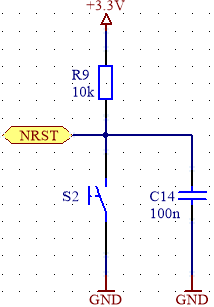
\includegraphics[width=.2\linewidth]{Schuh/Pictures/schaltung-reset}}\qquad
    \subfloat[Hardware\label{fig:coremodul-reset-hard}]{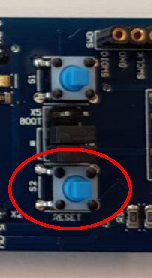
\includegraphics[width=.2\linewidth]{Schuh/Pictures/core-reset}}\qquad
    \caption[Reset-Schaltung des Core-Moduls]{Reset-Schaltung des \gls{Core-Modul}s}
    \label{fig:coremodul-reset}
\end{figure}

\subsubsection{5 V Spannungsversorgung}
Die \unit{+5}{\volt} Spannungsversorgung für das \gls{Core-Modul} kann auf zwei verschiedenen Wegen bezogen werden. Entweder man verwendet den ST-Link V2 Mini als \unit{5}{\volt} Spannungsversorgung X1 (\fref{fig:coremodul-swd}), wie bereits in \fref{sec:coremodul-stlink} beschrieben, oder man speist die \unit{+5}{\volt} Versorgung über den \unit{5}{\volt}-Pin des 50-poligen Headers des \gls{Core-Modul}s X2 (\fref{fig:coremodul-spannung}) ein.

\fig{coremodul-spannung}{Spannungsversorgungsschaltung des Core-Moduls}{Spannungsversorgungsschaltung des \gls{Core-Modul}s}{0.5\textwidth}{Schuh/Pictures/schaltung-spannung}

\subsubsection{Batterieversorgung}
Am VB-Anschluss des 50-poligen Headers (\fref{fig:coremodul-spannung}) kann eine \unit{3,3}{\volt}-Batterie angeschlossen werden, damit die \gls{RTC} auch dann mit Spannung versorgt ist, wenn der Cortex-M3 außer Betrieb ist. Darüber hinaus wird im Falle des stromsparenden Deep-Sleep-Mode des Cortex-M3 ebenfalls eine Puffer-Batterie benötigt. Die Schottky-Diode V4 (\fref{fig:coremodul-batterie}) soll verhindern, dass die Batterie welche die \gls{RTC} des Cortex betreiben soll, nicht geladen wird. In den meisten Fällen handelt es sich bei dieser Batterie um eine Knopfzelle, welche häufig nicht wiederaufladbar ist. Die Schottky-Diode V3 (\fref{fig:coremodul-batterie}) soll verhindern, dass die Batteriespannung der \unit{3,3}{\volt}-Knopfzelle, mit der über einen Linearregler generierten Versorgungsspannung des Prozessors verbunden wird.

\fig{coremodul-batterie}{Batterieversorgungsschaltung des Core-Moduls}{Batterieversorgungsschaltung des \gls{Core-Modul}s}{0.5\textwidth}{Schuh/Pictures/schaltung-batterie}

\subsubsection{3,3 V Fixspannungsregler}
Zur Generierung der für den Prozessor erforderlichen Betriebsspannung wurde ein \unit{3,3}{\volt}-Linearregler U2 (\fref{fig:coremodul-fix}) verwendet, welcher die Eingangsspannung von \unit{+5}{\volt} auf \unit{+3,3}{\volt} herabsetzt. Bei Verwendung eines Linearreglers ist zu beachten, dass dieser die Spannungsdifferenz zwischen Ausgangsspannung und Eingangsspannung in Wärme umwandelt. Daher sollten keine temperaturempfindlichen Bauteile in dessen Nähe platziert werden. Zur Überprüfung, ob das Modul mit der Betriebsspannung von \unit{+5}{\volt} versorgt wird, wurde die LED V5 (\fref{fig:coremodul-fix}) zur optischen Kontrolle eingebaut. Wenn das Modul mit Spannung versorgt wird, leuchtet diese. Zur Überprüfung ob der Prozessor mit seiner Betriebsspannung von \unit{3,3}{\volt} versorgt wird, wurde die LED V6 (\fref{fig:coremodul-fix}) zur optischen Kontrolle eingebaut. Wenn der Prozessor mit Spannung versorgt wird, leuchtet sie. Um den Stromverbrauch des \gls{Core-Modul}s im Low-Power Modus weiter zu senken, können die LEDs mit Hilfe von Jumpern außer Betrieb gesetzt werden.

\begin{figure}[htb]
    \centering
    \subfloat[Schematic\label{fig:coremodul-fix-schem}]{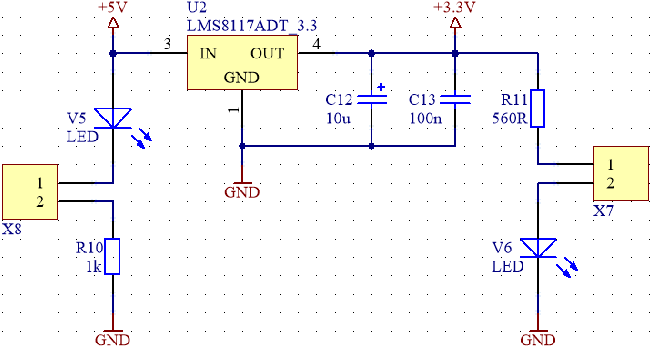
\includegraphics[width=.75\linewidth]{Schuh/Pictures/schaltung-fix}}\qquad
    \subfloat[Hardware\label{fig:coremodul-fix-hard}]{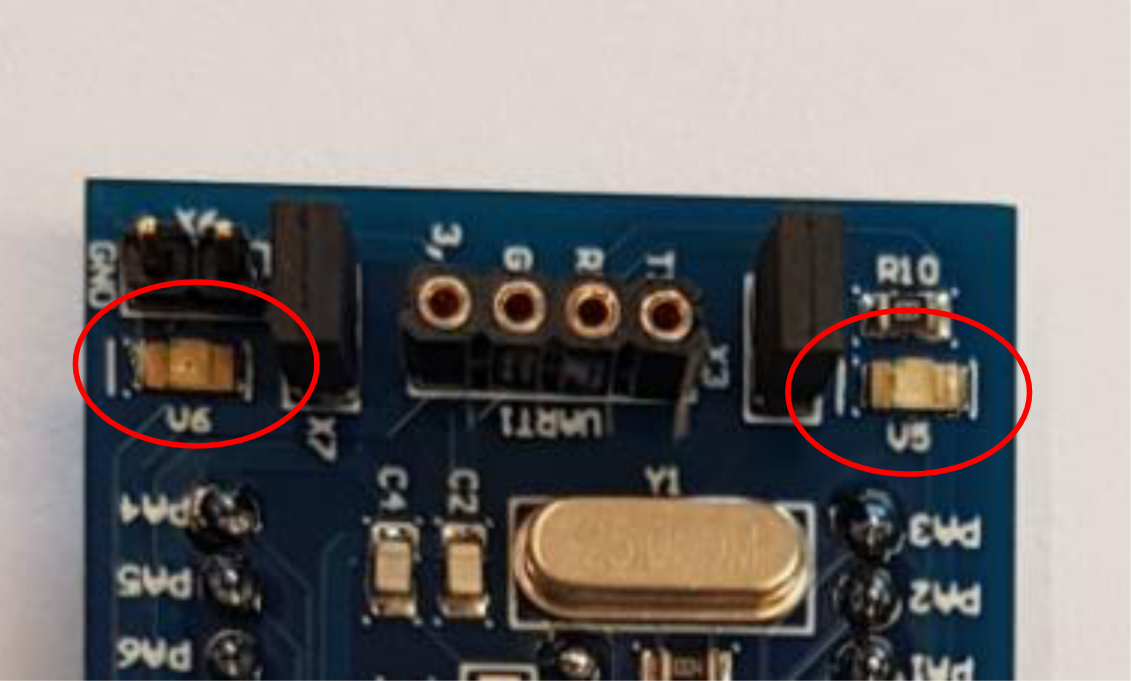
\includegraphics[width=.4\linewidth]{Schuh/Pictures/core-fix}}\qquad
    \caption[Fixspannungsregler des Core-Moduls]{Fixspannungsregler des \gls{Core-Modul}s}
    \label{fig:coremodul-fix}
\end{figure}


\subsubsection{Prozessor}
In \fref{fig:coremodul-prozessor} ist die Pinbelegung des verwendeten Prozessors U1 dargestellt.

\begin{figure}[H]
    \centering
    \subfloat[Schematic\label{fig:coremodul-prozessor-schem}]{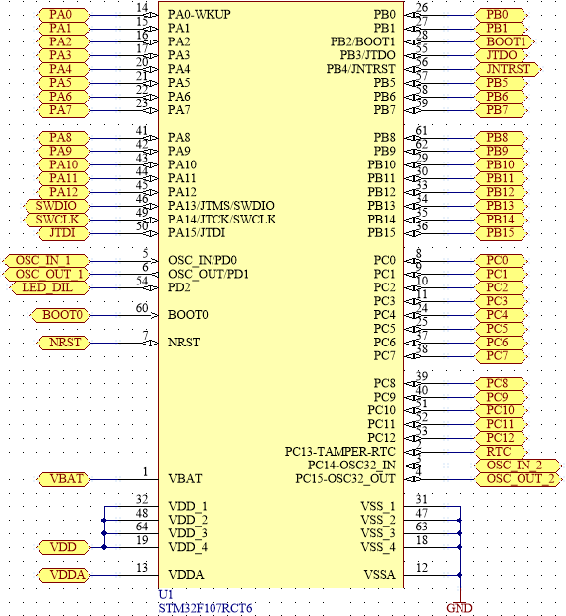
\includegraphics[width=.75\linewidth]{Schuh/Pictures/schaltung-prozessor}}\qquad
    \subfloat[Hardware\label{fig:coremodul-prozessor-hard}]{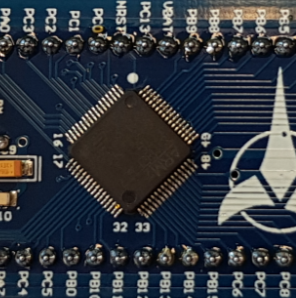
\includegraphics[width=.4\linewidth]{Schuh/Pictures/core-prozessor}}\qquad
    \caption[Prozessor des Core-Moduls]{Prozessor des \gls{Core-Modul}s}
    \label{fig:coremodul-prozessor}
\end{figure}

\subsubsection{Stützkondensatoren}
Während des laufenden Betriebs eines Microcontrollers benötigt dieser unterschiedlich viel Strom. Um Spannungseinbrüche zu vermeiden wurden die Stützkondensatoren C5, C6, C7 und C8 (\fref{fig:coremodul-kond}) vorgesehen. Die Stützkondensatoren können die in ihnen gespeicherte Ladung bei stark wechselnden Stromaufnahmen abgeben und somit eine ordnungsgemäße Versorgung des Prozessors gewährleisten.

\fig{coremodul-kond}{Stützkondensatoren des Core-Moduls}{Stützkondensatoren des \gls{Core-Modul}s}{0.5\textwidth}{Schuh/Pictures/schaltung-kond}

\subsubsection{DIL-Adapter}
Das Schaltplansymbol des DIL-Adapters X2 (\fref{fig:coremodul-dil}) zeigt das Pinning, welches hardwaremäßig auf den zwei getrennten Buchsenleisten auf der Leiterkarte ausgeführt wurde.

\fig{coremodul-dil}{DIL-Adapter des Core-Moduls}{DIL-Adapter des \gls{Core-Modul}s}{0.5\textwidth}{Schuh/Pictures/schaltung-dil}

\subsubsection{Schwingquarze}
Das \gls{Core-Modul} besitzt standardmäßig zwei verschiedene Taktquellen. Diese bestehen aus einem 25MHz Quarz Y1 (\fref{fig:coremodul-quarz}), welcher für die Taktfrequenz des Prozessors zuständig ist, und einem 32kHz Quarz Y2 (\fref{fig:coremodul-quarz}), welcher für die interne \gls{RTC} zur Verfügung steht.

\fig{coremodul-quarz}{Schwingquarze des Core-Moduls}{Schwingquarze des \gls{Core-Modul}s}{0.75\textwidth}{Schuh/Pictures/schaltung-quarz}

\subsubsection{Taster}
Auf dem \gls{Core-Modul} wurde ein Kurzhubtaster S1 (\fref{fig:coremodul-taster}) vorgesehen, dessen Funktion nach belieben ausprogrammiert werden kann.

\begin{figure}[htb]
    \centering
    \subfloat[Schematic\label{fig:coremodul-taster-schem}]{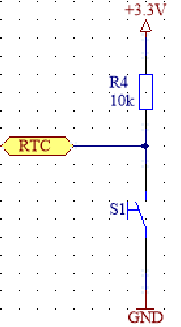
\includegraphics[width=.25\linewidth]{Schuh/Pictures/schaltung-taster}}\qquad
    \subfloat[Hardware\label{fig:coremodul-taster-hard}]{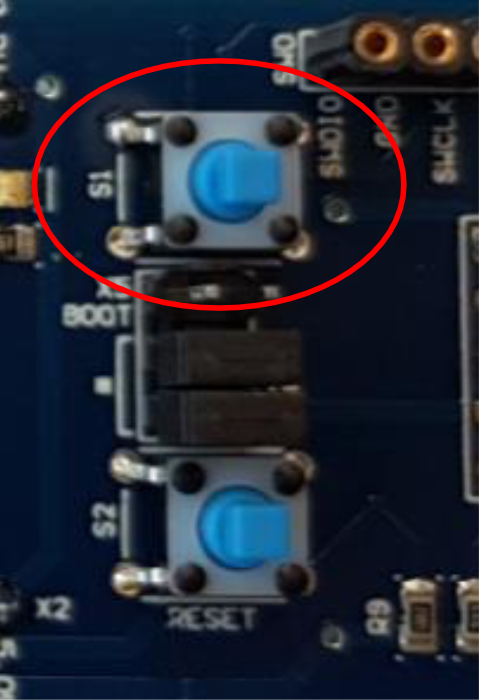
\includegraphics[width=.25\linewidth]{Schuh/Pictures/core-taster}}\qquad
    \caption[Taster des Core-Moduls]{Taster des \gls{Core-Modul}s}
    \label{fig:coremodul-taster}
\end{figure}

\subsubsection{LED}
Auf dem \gls{Core-Modul} wurde eine LED V2 (\fref{fig:coremodul-led}) vorgesehen, deren Funktion nach belieben ausprogrammiert werden kann.

\begin{figure}[htb]
    \centering
    \subfloat[Schematic\label{fig:coremodul-led-schem}]{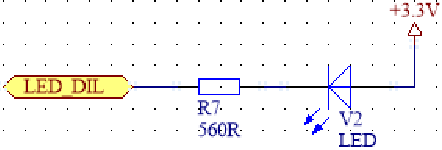
\includegraphics[width=.4\linewidth]{Schuh/Pictures/schaltung-led}}\qquad
    \subfloat[Hardware\label{fig:coremodul-led-hard}]{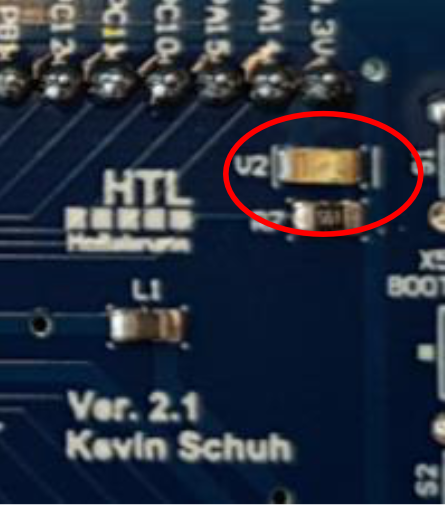
\includegraphics[width=.25\linewidth]{Schuh/Pictures/core-led}}\qquad
    \caption[LED des Core-Moduls]{LED des \gls{Core-Modul}s}
    \label{fig:coremodul-led}
\end{figure}

\subsubsection{Masseschleife}
Um das Messen mit einem Oszilloskop oder anderen Messgeräten zu vereinfachen wurde eine Masseschleife X6 (\fref{fig:coremodul-masse}) auf dem \gls{Core-Modul} vorgesehen.

\begin{figure}[htb]
    \centering
    \subfloat[Schematic\label{fig:coremodul-masse-schem}]{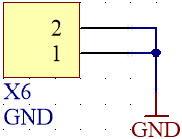
\includegraphics[width=.25\linewidth]{Schuh/Pictures/schaltung-masse}}\qquad
    \subfloat[Hardware\label{fig:coremodul-masse-hard}]{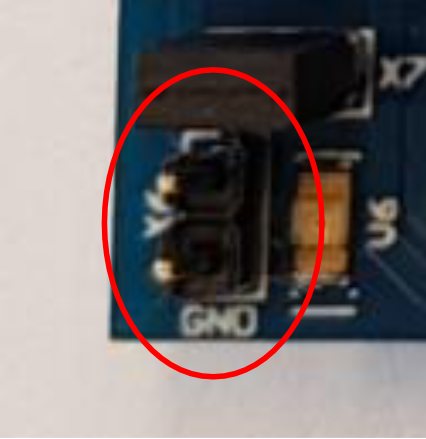
\includegraphics[width=.25\linewidth]{Schuh/Pictures/core-masse}}\qquad
    \caption[Masseschleife des Core-Moduls]{Masseschleife des \gls{Core-Modul}s}
    \label{fig:coremodul-masse}
\end{figure}

\subsection{Gesamtschaltung}
\label{sec:coremodul-schaltung}
\fig{coremodul-gesamtschaltung}{Gesamtschaltung des Core-Moduls}{Gesamtschaltung des \gls{Core-Modul}s}{0.8\textwidth}{Schuh/Pictures/SchaltungCM}

\subsection{Leiterplattenlayout}
\label{sec:coremodul-leiterplattenlayout}
\subsubsection{Bauteilseite}
\fig{coremodul-lbauteilseite}{Layout Bauteilseite des Core-Moduls}{Layout Bauteilseite des \gls{Core-Modul}s}{\textwidth}{Schuh/Pictures/core-lbauteilseite}

\subsubsection{Lötseite}
\fig{coremodul-llötseite}{Layout Lötseite des Core-Moduls}{Layout Lötseite des \gls{Core-Modul}s}{\textwidth}{Schuh/Pictures/core-llotseite}

\subsection{Bestückungspläne}
\label{sec:coremodul-bestückungspläne}
\subsubsection{Bauteilseite}
\fig{coremodul-bbauteilseite}{Bestückungsplan Bauteilseite des Core-Moduls}{Bestückungsplan Bauteilseite des \gls{Core-Modul}s}{\textwidth}{Schuh/Pictures/core-bbauteilseite}

\subsubsection{Lötseite}
\fig{coremodul-blötseite}{Bestückungsplan Lötseite des Core-Moduls}{Bestückungsplan Lötseite des \gls{Core-Modul}s}{\textwidth}{Schuh/Pictures/core-blotseite}